\section{Nota teórica}
En esta sección del laboratorio, se exponen los principales componentes que usarán para el proyecto a realizar: un voltímetro.
\subsection*{Arduino UNO}
Se usará la placa de Arduino UNO que posee el microcontrolador ATMega382P.

\subsubsection*{Características generales}
Sus detalles se describen a continuación:
\begin{itemize}
\item Es un MCU de 8 bits.
\item Posee arquitectura RISC/Harvard.
\item 4/8/16/64 kb memoria flash.
\item 512b/1/2kb de memoria SRAM.
\item 1/2kb de EEPROM.
\item 23 GPIOS.
\item Timer/Counters de 8 y 16 bits.
\item Posee interrupciones.
\item 8 canaels PWM y comparador analógico.
\item 6 canales 10-bit ADC.
\item Posee protocolo SPI y USART (Universal Synchronous/Asynchronous Receiver/Transmitter) I2C.
\end{itemize}
\subsubsection*{Diagrama de bloques y pines}
El diagrama de bloques de este MCU se muestra en la figura \ref{fig1}.

\begin{figure}[H]
\centering
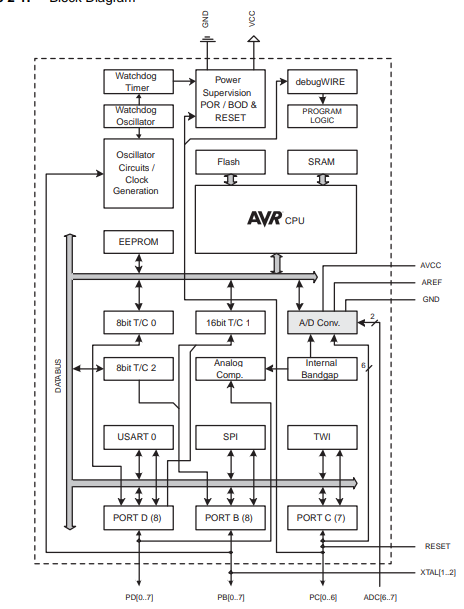
\includegraphics[width=.8\linewidth]{Imagenes/1.png}
 \caption{Diagrama de bloques de ATMega328P. Tomado de \cite{web1}.}
 \label{fig1}
\end{figure}

\begin{figure}[H]
\centering
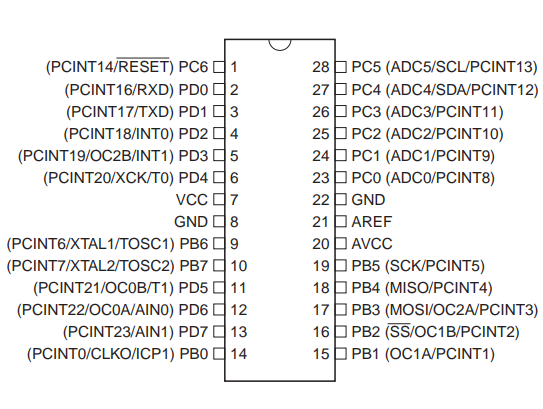
\includegraphics[width=.8\linewidth]{Imagenes/2.png}
 \caption{Diagrama de pines de ATMega328P. Tomado de \cite{web1}.}
 \label{fig2}
\end{figure}
Dado que será necesario saber a profundidad la clasificación de estos pines la figura \ref{fig2.1} brinda una mejor clasificación de éstos.
\begin{figure}[H]
\centering
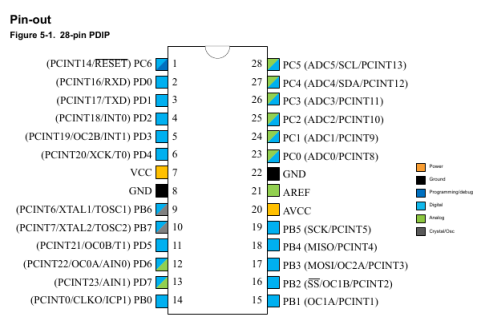
\includegraphics[width=.8\linewidth]{Imagenes/2.1.png}
 \caption{Clasificación de pines de ATMega328P. Tomado de \cite{web5}.}
 \label{fig2.1}
\end{figure}

\subsubsection*{Características eléctricas}
La siguiente lista describe estos detalles.
\begin{itemize}
\item Voltaje: 1.8-\SI{5.5}{\volt}.
\item Velocidad: 0-\SI{4}{\mega\Hz},  1.8-\SI{5.5}{\volt}. 0-\SI{10}{\mega\Hz},  2.7-\SI{5.5}{\volt}. 0-\SI{20}{\mega\Hz},  4.5-\SI{5.5}{\volt}
\item Modo activo: \SI{0.3}{\mA}
\item Temperatura de funcionamiento: $-55^\circ$ a +$125^\circ$.
\item Temperatura de almacenamiento: $-65^\circ$ a +$125^\circ$.
\item Temperatura pin RESET y GND: -\SI{0.5}{\volt} a \SI{13}{\volt}.
\item Temperatura en los demás pines: -\SI{0.5}{\volt} a VCC\SI{0.5}{\volt}.
\item Corriente por pin I/O: \SI{40}{\mA}.
\end{itemize}
Sabiendo lo anterior, resulta pertinente mencionar la descripción de los pines usados en este laboratorio. Para la conexión de las fuentes de DC y AC, se usaron los pines \texttt{A5, A4, A3, A2}. Que se caracterizan por ser entre analógicos y digitales, esto permite tener más facilidad en cuanto a funciones. Mismo escenario para el botón de modo AC, solo que en este caso está conectado al pin \texttt{A0}. En cuanto a los pines que activan las alarmas de los LEDs y los que se conectaron a la pantalla PCD8544 se han usado los que son totalmente digitales (11-3), es decir, estos pines solo pueden funcionar como salidas o entradas, por lo que se declaron como \texttt{INPUT} o \texttt{OUTPUT}. Por último, para la comunicación serial se usaron los pines \texttt{RX} y \texttt{TX}, ya que son los encargados de la comunicación.
\subsection*{Periféricos utilizados}
Algunos periféricos usados del microcontrolador así como la pantalla PCD8544 fueron los siguientes:
\begin{itemize}
\item \textbf{pinMode:} esto se usó para cual pin era una entrada o salida, y esto ayuda para que el microcontrolador entienda todas las acciones que se desea realizar.
\item \textbf{digitalWrite:} básicamente su función es para establecer el estado de una variable después de una acción, típicamente es para poner en alto o en bajo una señal.
\item \textbf{analogRead:} esto devuelve el valor leído del pin de entrada analógico, el valor es proporcional a la entrada analógica tomando como base una tensión de referencia: 0-1023.
\item \textbf{display.begin:} inicia/enciende la pantalla.
\item \textbf{display.setContrast:} configuración del contraste de la pantalla.
\item \textbf{display.clearDisplay:} limpia la pantalla.
\item \textbf{display.setTextSize:} configura la posición del texto.
\item \textbf{display.setTextColor:} establece el color de las letras.
\item \textbf{display.setCursor:} este parámetro sirve para posicionar el texto en la pantalla.
\item \textbf{display.println:} imprime el contenido deseado.
\item \textbf{display.display:} imprime el logo de Adafruit y se coloca después de cada texto, de lo contrario no se mostrará el contenido.
\end{itemize}
Si bien, se debe mencionar que la pantalla PCD8544 desempeña un papel importante en este trabajo, porque permite mostrar las magnitudes de las tensiones eléctricas en las fuentes de alimentación, tanto para modo DC como AC. Por tanto, hay que conocer los pines que se usaron para darle sentido a los pererféricos mencionados anteriormente. En el simulador se tienen 5 pines que se explican a continuación \cite{web2}.
\begin{itemize}
\item \textbf{RST:} esta señal reiniciará el dispositivo y debe ser aplicado adecuadamente al chip. La señal activa está en bajo.
\item \textbf{CS:} habilita la pantalla con el que se está comunicando en un bus SPI. Cuando esta señal está activa, el PCD8544 está habilitado y listo para recibir comandos o datos a través del bus SPI. Cuando la señal CS está inactiva, la pantalla no responde y no acepta datos.
\item \textbf{D/C:} selecciona el modo de operación, alto o bajo.
\item \textbf{DIN:} es una entrada para la línea de datos.
\item \textbf{CLK:} es la señal de reloj que va de 0.0 a 4.0 Mbit/s.
\end{itemize}
Por lo que, los datos que se muestran en la pantalla PCD8544 es porque se usa el modelo de comunicaciones SPI: \texttt{Serial Peripheral Interface}, es un bus de interfaz comúnmente utilizado para enviar datos entre microcontroladores y pequeños periféricos como registros de desplazamiento, sensores y tarjetas SD \cite{web3}.
\subsection*{Componentes electrónicos complementarios}
Algunos de los componentes extra que fueron de gran ayuda para el diseño del voltímetro fueron los siguientes:
\begin{itemize}
\item Amplificadores inversores: se optó por esta opción, ya que el voltaje de salida de este tipo de amplificadores tienen la siguiente expresión:
\begin{equation}
v_o=-v_i\cdot \frac{R_2}{R1}
\label{eq1}
\end{equation}
Esto sirvió para diseñar que los rangos de tensión eléctrica no fueron mayores a \SI{5}{\volt}. De esa manera, la base para lograr esto fue con valores de $R_1=R_2=\SI{2.5}{\ohm}$ y $v_i=\SI{-2.5}{\volt}$,
\begin{figure}[H]
\centering
 \begin{circuitikz} \draw
 (0,0) node[op amp] (opamp) {}
 (opamp.+) node[left] {} node[ground] {}
 (opamp.-) node[left] {}
 (opamp.-) node[left] {}
 (opamp.out) node[right] {$v_o$};
 %\draw (0,0)--(opamp.-);
 \draw (-3,0.5) to[R=$R_1$,-*](opamp.-);
 \draw (-4,0.5)node[above]{$v_i$} to [short, o-](-3,0.5);
 \draw (opamp.-)--(-1.2,2.2)to[R=$R_2$](1.1, 2.2)to[short, -*](1.1,0);
\end{circuitikz}
\caption{Amplificador inversor.}
 \label{ampOp}
\end{figure}

A partir, del esquemático anterior y la fórmula \ref{eq1} fue posible regular las fuentes de tensión AC/DC para los 4 canales con el objetivo de obtener las mejores aproximaciones con respecto al voltímetro y lo mostrado en la pantalla.
\item Relay: en este componente se conectan las 8 entradas de las fuentes AC/DC y salen 4 que están conectadas a los amplificadores inversores, la idea es determinar cuando las fuentes AC y DC estén normalmente cerradas o normalmente abiertas.
\item Switches: son de gran ayuda para definir en que estado opera el voltímetro, si está realizando mediciones en AC o en DC, para realizar correctas lecturas de este cambio se debe tener en cuenta el diseño previo de valores de resistencia y capacitancia para evitar falsas lecturas. 
\begin{figure}[H]
\centering
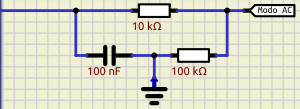
\includegraphics[width=.8\linewidth]{Imagenes/3.1.png}
 \caption{Diseño antirebote.}
 \label{fig3.1}
\end{figure}
El diseño anterior, ayuda a que la transición de DC a AC sea inmediata.
\end{itemize}

\subsection*{Lista de componentes}
La siguiente tabla resume los componentes (con sus precios) utilizados para este trabajo. La lista de precios mostrados en la tabla \ref{table_2} se tomaron de \cite{web4}. %FALTA AGREGAR LO RESTANTE DE LA COMUNICACION SERIAL.
\begin{table}[H]
\caption{Lista de equipos}
\label{table_2}
\begin{center}
\begin{tabular}{r|cc}
\hline
\textbf{Componente}&\textbf{Cantidad}&\textbf{Precio}\\
 \hline
Arduino UNO&1   &17\$ \\ \hline 
Kit de resistencias &1   &9.99\$ \\ \hline 
Capacitancias&1   &0.2\$ \\ \hline 
LEDs&4   &2.2\$ \\ \hline 
Pantalla PCD8544&1   &5.85\$ \\ \hline 
Botón&9   &5.85\$ \\ \hline 
Amplificadores&4   &3.8\$ \\ \hline 
RelaySPST & 2 & 29\$ \\ \hline 
Fuente de voltaje AC/DC& 1&48.95\$\\ \hline 

 \textbf{Total}& &  122.84\\
 \hline
\end{tabular}
\end{center}
\end{table}

\subsection*{Diseño del circuito}
El circuito que simula el voltímetro se muestra en la figura \ref{fig3}.
\begin{figure}[H]
\centering
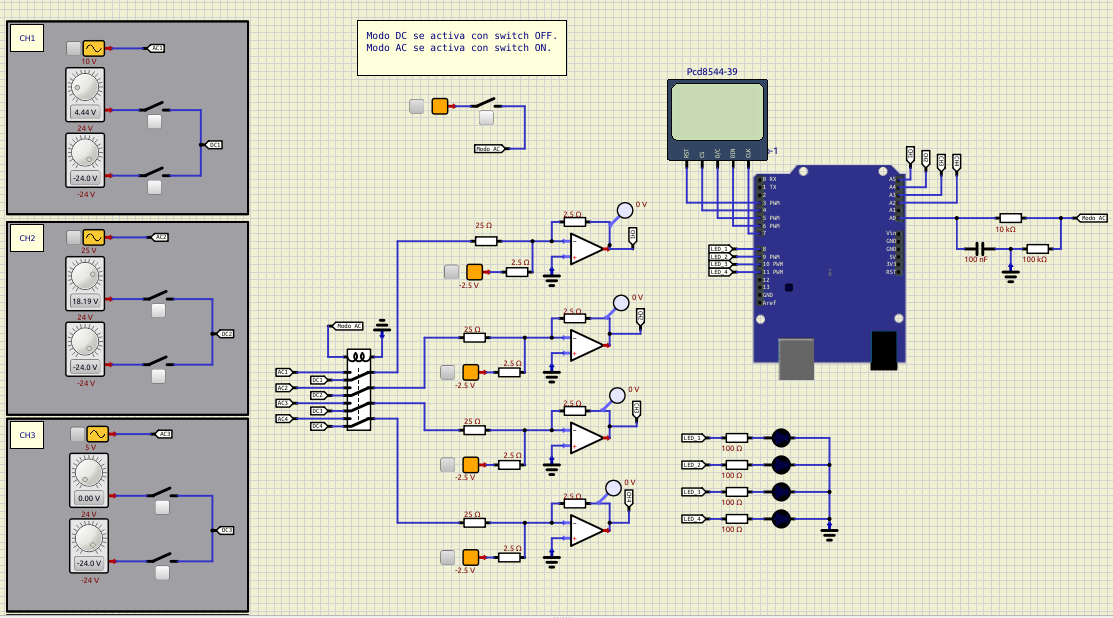
\includegraphics[width=.8\linewidth]{Imagenes/7.png}
 \caption{Circuito del voltímetro}
 \label{fig3}
\end{figure}
Inicialmente, se hizo uso del amplificador inversor para lograr obtener una magnitud de tensión eléctrica adecuada y así no sobrepasar el umbral del arduino. Tal como se mostró en la sección de componentes complementarios, tomar esos valores de resistencias y elegir un voltaje de magnitud negativa dará un valor adecuado que permita colocar fuentes de tensión para el buen funcionamiento del voltímetro. 
\begin{figure}[H]
\centering
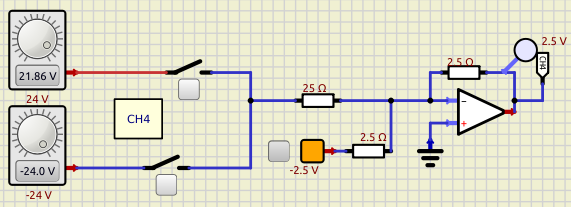
\includegraphics[width=.8\linewidth]{Imagenes/4.png}
 \caption{Tensión de salida a medir.}
 \label{fig4}
\end{figure}
Esto se realizó para los 4 canales que se van usar, los cuales se conectaron como entradas al arduino en los pines \texttt{A5-A2}. Luego, en los pines 7-3 se conectaron las señales \texttt{CLK, DIN, D/C, CS, RST} respectivamente, esto para realizar unas pequeñas pruebas de funcionamiento de la pantalla mostrando un pequeño mensaje para comprobar su correcta conexión. En la sección de resultados se darán más detalles de este diseño.
\begin{figure}[H]
\centering
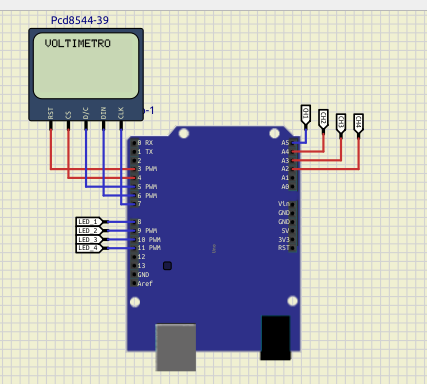
\includegraphics[width=.8\linewidth]{Imagenes/5.png}
 \caption{Funcionamiento correcto de la pantalla PCD8544.}
 \label{fig5}
\end{figure}
Después, la conexión de los LEDs de alarma al arduino en los pines 8-11 que fueron configurados como salidas, se van a encender cuando se supere el rango de -20 a 20 en DC, y -14.14 a 14.14 en AC.
\begin{figure}[H]
\centering
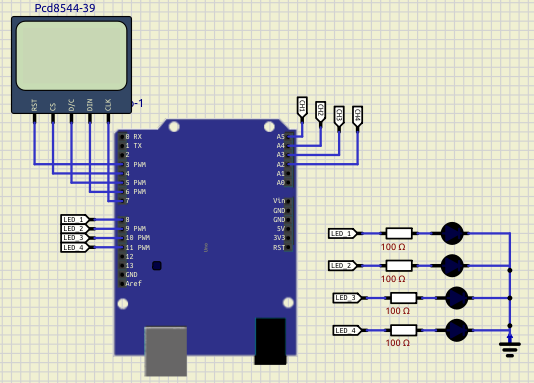
\includegraphics[width=.8\linewidth]{Imagenes/6.png}
 \caption{Conexión de los LEDs al arduino.}
 \label{fig6}
\end{figure}
Otro detalle, para ordenar el voltímetro se decidió usar un relay que sirve de puente entre las fuentes AC/DC y la salida de los amplificadores inversores que se comunicará con la PCD8544, la cual mostrará las tensiones eléctricas en AC (si el botón está en alto) o en DC, enviará señales a los LEDS y estos se pondrán en alto o no dependiendo de las magnitudes que tengan las fuentes variables de tensión y reflejadas en la PCD8544. Esto se ve de la siguiente manera \footnote{Por resolución de la imagen solo se mostrarán 3, en realidad posee 4.}.
\begin{figure}[H]
\centering
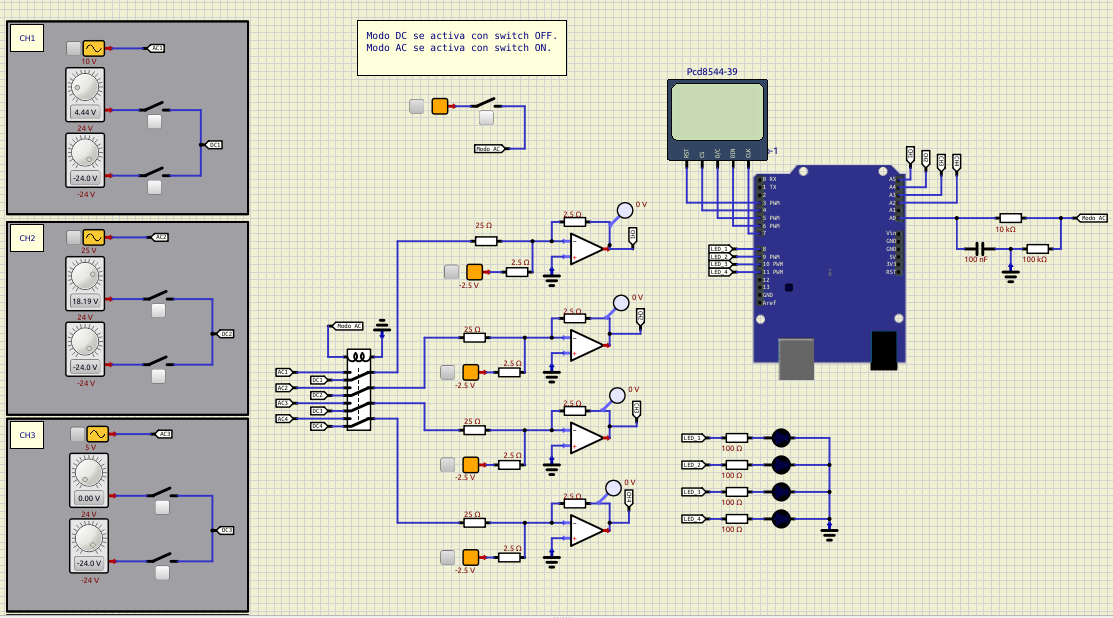
\includegraphics[width=.8\linewidth]{Imagenes/7.png}
 \caption{Canales del voltímetro.}
 \label{fig7}
\end{figure}
Ahora, para la comunicación serial se introduce un puerto serial encargado de realizar la comunicación entre el arduino y el puerto serial, también se hace uso de un relé para hacer cumplir con lo solicitado de que la transmisión se pueda controlar por medio de un switch, el resultado final se observa en la siguiente figura:
\begin{figure}[H]
    \centering
    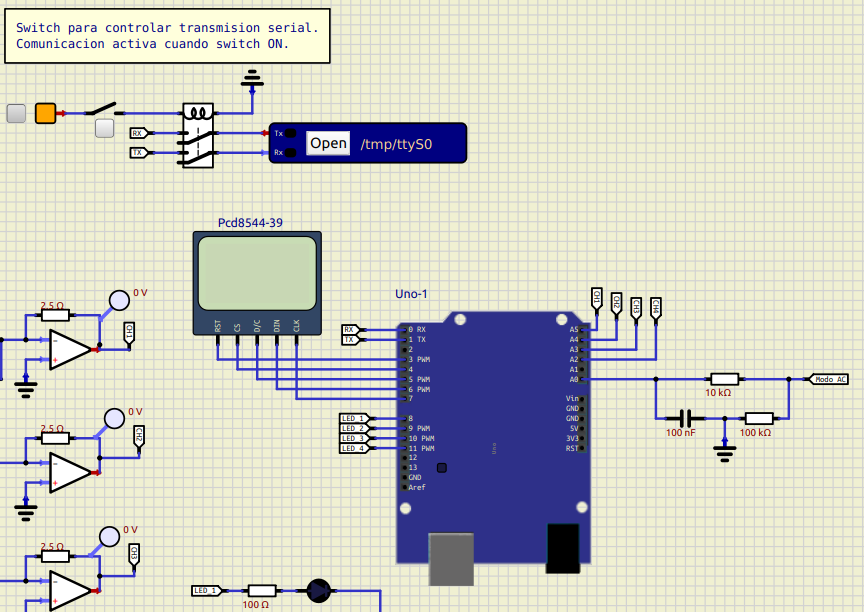
\includegraphics[width=.8\linewidth]{Imagenes/8.png}
    \caption{Introducción del puerto serial y el switch para realizar la comunicación.}
    \label{figk1}
\end{figure}

Es importante cuando se hace la conexión ver que se toma el RX de un puerto y se conecta con el puerto TX para que se pueda dar la comunicación como se vio en clases.
\newpage
